\section{PGM to CNF}

\subsection{ENC 1}
Our ENC1 encoding for the Cancer Bayesian network can be found in appendix~\ref{ENC1}.

\subsection{ENC 2}
Our ENC2 encoding for the Cancer Bayesian network can be found in appendix~\ref{ENC2}.



\section{SRL to CNF}
\subsection{Encoding of Monty Hall as CNF}
An encoding of problog programs can be generated by our program as follows:
\begin{lstlisting}
python3 scripts/inference.py --problog_file files/problog/monty_hall.pl
\end{lstlisting}
The CNF will be shown using the program's predicates. A version of the CNF in dimacs format will be shown as well.
See \texttt{README.MD} for more information.

Our CNF encoding for the given Monty Hall ProbLog program is:
\begin{align*}
    \land & (open\_door(2) \lor prize(2) \lor prize(3) \lor \neg p\_open\_door(2)\_0) \\
    \land & (open\_door(2) \lor prize(2) \lor \neg prize(3))                          \\
    \land & (\neg open\_door(2) \lor \neg prize(2) \lor \neg prize(2))                \\
    \land & (\neg open\_door(2) \lor \neg prize(2) \lor prize(3))                     \\
    \land & (\neg open\_door(2) \lor \neg prize(3) \lor \neg prize(2))                \\
    \land & (\neg open\_door(2) \lor \neg prize(3) \lor prize(3))                     \\
    \land & (\neg open\_door(2) \lor p\_open\_door(2)\_0 \lor \neg prize(2))          \\
    \land & (\neg open\_door(2) \lor p\_open\_door(2)\_0 \lor prize(3))               \\
    \land & (open\_door(3) \lor prize(2) \lor prize(3) \lor \neg p\_open\_door(3)\_0) \\
    \land & (open\_door(3) \lor prize(3) \lor \neg prize(2))                          \\
    \land & (\neg open\_door(3) \lor \neg prize(2) \lor \neg prize(3))                \\
    \land & (\neg open\_door(3) \lor \neg prize(2) \lor prize(2))                     \\
    \land & (\neg open\_door(3) \lor \neg prize(3) \lor \neg prize(3))                \\
    \land & (\neg open\_door(3) \lor \neg prize(3) \lor prize(2))                     \\
    \land & (\neg open\_door(3) \lor p\_open\_door(3)\_0 \lor \neg prize(3))          \\
    \land & (\neg open\_door(3) \lor p\_open\_door(3)\_0 \lor prize(2))               \\
    \land & (win\_keep \lor \neg prize(1))                                            \\
    \land & (\neg win\_keep \lor prize(1))                                            \\
    \land & (win\_switch \lor \neg prize(2) \lor open\_door(2))                       \\
    \land & (win\_switch \lor \neg prize(3) \lor open\_door(3))                       \\
    \land & (\neg win\_switch \lor prize(2) \lor prize(3))                            \\
    \land & (\neg win\_switch \lor prize(2) \lor \neg open\_door(3))                  \\
    \land & (\neg win\_switch \lor \neg open\_door(2) \lor prize(3))                  \\
    \land & (\neg win\_switch \lor \neg open\_door(2) \lor \neg open\_door(3))        \\
    \land & (\neg prize(1) \lor \neg prize(2))                                        \\
    \land & (\neg prize(1) \lor \neg prize(3))                                        \\
    \land & (\neg prize(2) \lor \neg prize(3))                                        \\
    \land & (prize(1) \lor prize(2) \lor prize(3))\\
    & \textbf{Weights:}             \\
    & W(p\_open\_door(2)\_0) = 0.5 \\
    & W(p\_open\_door(3)\_0) = 0.5 \\
    & W(select\_door(1)) = 1.00    \\
    & W(prize(1)) = 0.33           \\
    & W(prize(2)) = 0.33           \\
    & W(prize(3)) = 0.33           \\
    & W(open\_door(2)) = 1.00      \\
    & W(open\_door(3)) = 1.00      \\
    & W(win\_keep) = 1.00          \\
    & W(win\_switch) = 1.00        \\
\end{align*}


\section{Weighted Model Counting}
\subsection{Weighted model counters on above CNFs}
We will use MiniC2D and Cachet as WMC counters.

\subsubsection{MiniC2D}
MiniC2D needs to use the $-W$ option to do weighted model counting.
\begin{itemize}
	\item ENC1:
\begin{figure}[H]
  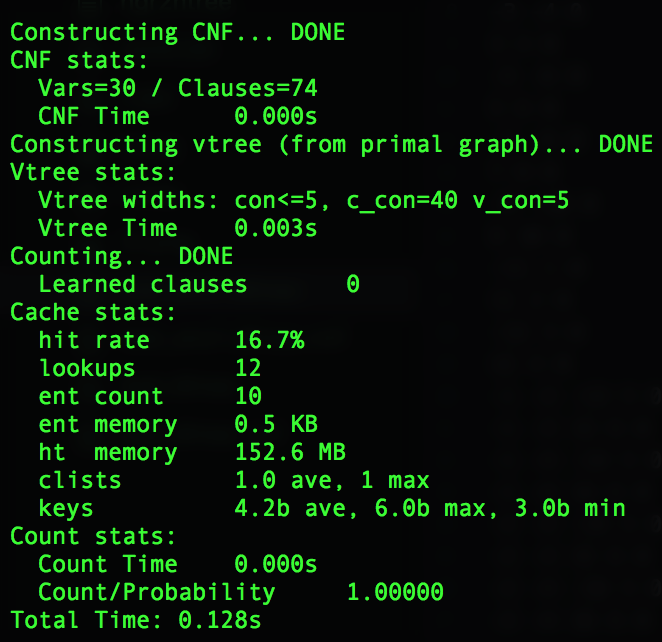
\includegraphics[width=6cm]{minic2d-ENC1.png}
  \caption{Grounded problog cnf}
\end{figure}
	\item ENC2:
	\begin{figure}[H]
  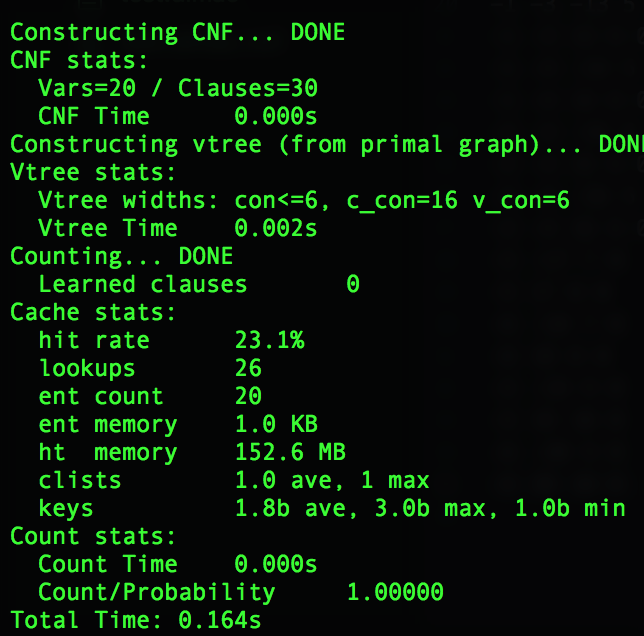
\includegraphics[width=6cm]{minic2d-ENC2.png}
  \caption{Grounded problog cnf}
\end{figure}
	\item Prolog first:
\end{itemize}

\subsubsection{Cachet}
\begin{itemize}
	\item ENC1: 
\begin{figure}[H]
\begin{center}
  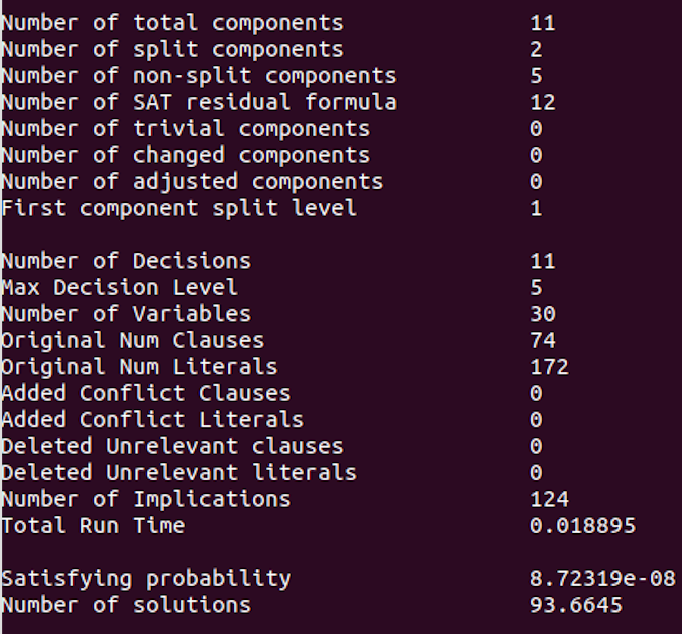
\includegraphics[width=5cm]{cachet-ENC1.png}
  \caption{Grounded problog cnf}
\end{center}
\end{figure}
	\item ENC2:
\begin{figure}[H]
\begin{center}
  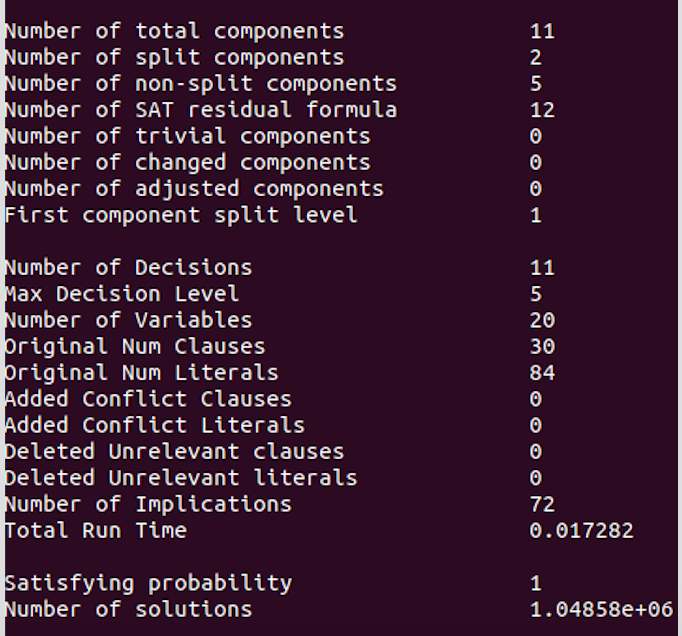
\includegraphics[width=5cm]{cachet-ENC2.png}
  \caption{Grounded problog cnf}
\end{center}
\end{figure}
	\item Prolog first:
\end{itemize}
For ENC1 we see that with Cachet we get a satisfying probability of almost $0$. This is due to the fact that with ENC1 all our negative literals have a weight of 1, while Cachet expects that a literal $+$ its negation $= 1$. 
\subsection{Difference between the selected WMCs}
%The differences between the different WMCs come from \cite{CHAVIRA2008772}.
%\subsubsection{Cachet vs jointree and recursive conditioning}
%Jointree and recursive conditioning only exploit topological structure thus they take no advantage of the massive determinism available in networks whilst Cachet does this.

\subsubsection{MiniC2D Vs Cachet}
MiniC2D and Cachet are both weighted model counters but how to do this is quite different.
MiniC2D is a top down compiler that compiles CNFs into a SDD which results in a faster system but it also uses less space while Cachet is an algorithm that uses formula caching together with clause learning and component analysis. MiniC2D needs vtrees to be able to compile the CNFs into an SDD.
T%he former is thus a compiler that uses SDDs while the other isn't.
They, however, both use things from the SAT literature. 
They both use clause learning and component caching as to be able to reuse components that later appear again in the search. Cachet on the other hand also uses some other things from SAT literature like an explicit on the fly calculation of connected components. This is different in MiniC2D as it uses a vtree to identify disconnected CNF components.
%The way that the compilation is done with MiniC2D is as follows:
%The SDD compilation is driven by the vtree, it uses this to identify disconnected CNF components and it uses a component caching scheme to prevent compiling the same component multiple times.
\cite{MiniC2D} \cite{Cachet}
%\subsubsection{ACE Vs Cachet}
%The biggest difference between them is that Cachet is a WMC by search and ACE is a WMC by compilation. In \cite{CHAVIRA2008772} they say that ACE and Cachet are almost equal in speed. They mention that they had to dissable some of ACE's built-in ways to optimze the search to make the comparisson fair. It can for example encode equal parameters, use structured resolutions, eclauses, ... \cite{CHAVIRA2008772} which optimize the search.
%They also differ in some other ways like the way they do decompositions, variable splitting and caching \cite{CHAVIRA2008772}.
%In \cite{CHAVIRA2008772} they note though that by enabling all the speed up features ACE has, that it is not always faster than Cachet.

\subsection{Overview of computational requirements}
All the tests can be found in the test folder.
We used our scripts to create the dimac files. The input files for our enc1 and enc2 converter ard ``.dsc'' files which can be found at 
\url{http://www.bnlearn.com/bnrepository/discrete-small.html#cancer}.

\subsubsection{Test 1: Cancer network}
\begin{table}[H]
\centering
\caption{My caption}
\label{my-label}
\begin{tabular}{c|c|c|c|c|c|c|}
\cline{2-7}
        & \multicolumn{3}{c|}{ENC1} & \multicolumn{3}{c|}{ENC2} \\ \cline{2-7} 
  & \textbf{Prob}  & \textbf{Memory}  & \textbf{Runtime} & \textbf{Prob}  & \textbf{Memory}  & \textbf{Runtime} \\ \cline{1-7} 
  \textbf{Minic2d} & 1.0  & 0.2 KB    & 0.155s   & 1.0    & 1.0 KB    & 0.000s \\
  \hline
\textbf{Cachet}  & val1  & val2    & a       & b     & val3    & val4    \\ \cline{1-7} 
\end{tabular}
\end{table}

\subsubsection{Test 2: asia network}
\begin{table}[H]
\centering
\caption{My caption}
\label{my-label}
\begin{tabular}{c|c|c|c|c|c|c|}
\cline{2-7}
        & \multicolumn{3}{c|}{ENC1} & \multicolumn{3}{c|}{ENC2} \\ \cline{2-7} 
  & \textbf{Prob}  & \textbf{Memory}  & \textbf{Runtime} & \textbf{Prob}  & \textbf{Memory}  & \textbf{Runtime} \\ \cline{1-7} 
  \textbf{Minic2d} & 1.0  & 0.9 KB    & 0.145s   & 1.0    & 2.0 KB    & 	 0.139s \\
  \hline
\textbf{Cachet}  & val1  & val2    & a       & b     & val3    & val4    \\ \cline{1-7} 
\end{tabular}
\end{table}

\subsubsection{Test 3: sachs network}
\begin{table}[H]
\centering
\caption{My caption}
\label{my-label}
\begin{tabular}{c|c|c|c|c|c|c|}
\cline{2-7}
        & \multicolumn{3}{c|}{ENC1} & \multicolumn{3}{c|}{ENC2} \\ \cline{2-7} 
  & \textbf{Prob}  & \textbf{Memory}  & \textbf{Runtime} & \textbf{Prob}  & \textbf{Memory}  & \textbf{Runtime} \\ \cline{1-7} 
  \textbf{Minic2d} & 0.99707  & 14.3 KB    & 0.184s   & 1.0    & 14.5 KB   & 	0.154s \\
  \hline
\textbf{Cachet}  & val1  & val2    & a       & b     & val3    & val4    \\ \cline{1-7} 
\end{tabular}
\end{table}

\subsubsection{Test 4: earthquake network}
\begin{table}[H]
\centering
\caption{My caption}
\label{my-label}
\begin{tabular}{c|c|c|c|c|c|c|}
\cline{2-7}
        & \multicolumn{3}{c|}{ENC1} & \multicolumn{3}{c|}{ENC2} \\ \cline{2-7} 
  & \textbf{Prob}  & \textbf{Memory}  & \textbf{Runtime} & \textbf{Prob}  & \textbf{Memory}  & \textbf{Runtime} \\ \cline{1-7} 
  \textbf{Minic2d} & 1.0  & 0.6 KB & 0.137s   & 1.0    & 1.0 KB  & 	0.153s \\
  \hline
\textbf{Cachet}  & val1  & val2    & a       & b     & val3    & val4    \\ \cline{1-7} 
\end{tabular}
\end{table}

\subsubsection{Test 5: survey network}
\begin{table}[H]
\centering
\caption{My caption}
\label{my-label}
\begin{tabular}{c|c|c|c|c|c|c|}
\cline{2-7}
        & \multicolumn{3}{c|}{ENC1} & \multicolumn{3}{c|}{ENC2} \\ \cline{2-7} 
  & \textbf{Prob}  & \textbf{Memory}  & \textbf{Runtime} & \textbf{Prob}  & \textbf{Memory}  & \textbf{Runtime} \\ \cline{1-7} 
  \textbf{Minic2d} & 1.0  & 1.6 KB    & 0.125s   & 1.0    & 2.0 KB    & 	0.125s \\
  \hline
\textbf{Cachet}  & val1  & val2    & a       & b     & val3    & val4    \\ \cline{1-7} 
\end{tabular}
\end{table}

\subsubsection{Test 6: alarm network}
\begin{table}[H]
\centering
\caption{My caption}
\label{my-label}
\begin{tabular}{c|c|c|c|c|c|c|}
\cline{2-7}
        & \multicolumn{3}{c|}{ENC1} & \multicolumn{3}{c|}{ENC2} \\ \cline{2-7} 
  & \textbf{Prob}  & \textbf{Memory}  & \textbf{Runtime} & \textbf{Prob}  & \textbf{Memory}  & \textbf{Runtime} \\ \cline{1-7} 
  \textbf{Minic2d} & 1.0  & 959.7KB KB    & 0.268s   & 1.0    & 139KB    & 	0.095s \\
  \hline
\textbf{Cachet}  & val1  & val2    & a       & b     & val3    & val4    \\ \cline{1-7} 
\end{tabular}
\end{table}

\subsubsection{Test 6: andes network}
\begin{table}[H]
\centering
\caption{My caption}
\label{my-label}
\begin{tabular}{c|c|c|c|c|c|c|}
\cline{2-7}
        & \multicolumn{3}{c|}{ENC1} & \multicolumn{3}{c|}{ENC2} \\ \cline{2-7} 
  & \textbf{Prob}  & \textbf{Memory}  & \textbf{Runtime} & \textbf{Prob}  & \textbf{Memory}  & \textbf{Runtime} \\ \cline{1-7} 
  \textbf{Minic2d} & 1.0  & 2.7GB    & 122.78s   & 1.0    & 139.8MB    & 	6.086s \\
  \hline
\textbf{Cachet}  & val1  & val2    & a       & b     & val3    & val4    \\ \cline{1-7} 
\end{tabular}
\end{table}



\section{Knowledge compilation}
\subsubsection{Vtree with the most compact circuit}

\subsubsection{Pattern for a good vtree}

